\section{Předtermín 10. ledna 2025}

\subsection{Rozvin řady}
Rozviňte funkci $f(x) = \frac{x}{1+2x^2}$ se středem v $x_0 = 0$ do mocninné řady. Určete největší otevřený interval, kde 
nastává rovnost funkce a řady.

\subsection{Stacionární body}
Vyšetřete stacionární body funkce $f(x) = 2x^2 - x^4 - 2y^2 + 4xy - 1$.

Funkce je polynom a tedy má derivace všech řádů. Nutnou podmínkou pro extrém v daném bodě je nulovost první derivace.

$$\dif f(x, y) = (4x - 4x^3 + 4y, -4y + 4x)$$

Tedy $\dif f(x, y) = 0$ $\iff$ $x=y \land x(2-x^2) = 0$, což je právě když $(x,y)=(0,0)$ nebo $(x,y)=\pm(\sqrt{2},\sqrt{2})$.

V těchto kritických bodech dále vyšetříme druhou derivaci:
$$\dif^2 f(x,y)=
    \begin{bmatrix}
        4-12x^2 & 4\\
        4 & -4
    \end{bmatrix}
$$

\begin{itemize}
    \item Pro $(x,y) = (0,0)$ je $\dif^2f(0,0) = 
        \begin{bmatrix}
            4 & 4\\
            4 & -4
        \end{bmatrix}
        $. Podle Sylvestrova kritéria ($\Delta_1 = 4>0, \Delta_2 = -32 < 0$) je forma indefinitní, a tedy v daném bodě 
        je sedlový bod.
    \item Pro $(x,y) = (\sqrt{2}, \sqrt{2})$ je $\dif^2f(\sqrt{2}, \sqrt{2}) = 
    \begin{bmatrix}
        -20 & 4\\
        4 & -4
    \end{bmatrix}
    $. Podle Sylvestrova kritéria ($\Delta_1 = -20<0, \Delta_2 = 64 > 0$) je forma negativně definitní, a tedy v daném bodě 
    je MAXIMUM.
    \item Pro $(x,y) = (-\sqrt{2}, -\sqrt{2})$ je $\dif^2f(-\sqrt{2}, -\sqrt{2}) = 
    \begin{bmatrix}
        -20 & 4\\
        4 & -4
    \end{bmatrix}
    $. Podle Sylvestrova kritéria ($\Delta_1 = -20<0, \Delta_2 = 64 > 0$) je forma negativně definitní, a tedy v daném bodě 
    je MAXIMUM.
\end{itemize}

\subsection{Práce síly vektorového pole}
Ukažte, že práce síly $\vec{F} = (2xz + \sin y, x \cos y + z, x^2+y)$ podél křivky z $[0, 1, 0]$ do $[1, 0, 1]$ nezávisí
na křivce a najděte její hodnotu.

\subsection{Dvojný integrál}
Přepište následující integrál
\[
\int_{-1}^1 \int_{1 - \sqrt{1-y^2}}^{1 + \sqrt{1-y^2}} f(x, y) \dif x \dif y
\]
\begin{enumerate}[a), noitemsep]
    \item v opačném pořadí integrace,
    \item v polárních souřadnicích se středem v počátku v pořadí $\dif \varrho \dif \varphi$.
\end{enumerate}

\begin{multicols}{2}
    Opačné pořadí:
    \begin{flalign*}
        E\text{: } &0 \leq x \leq 2 & \\
        &- \sqrt{1-(x-1)^2} \leq y \leq \sqrt{1-(x-1)^2}
    \end{flalign*}
    $$\int_{0}^{2} \int_{- \sqrt{1-(x-1)^2}}^{\sqrt{1-(x-1)^2}} f(x,y) \dif y \dif x$$

    Polární souřadnice:
    \begin{flalign*}
        E\text{: } -\pi &\leq \varphi \leq \pi & \\
        0 &\leq \varrho \leq 2 \cos \varphi
    \end{flalign*}
    $$\int_{-\pi}^{\pi} \int_{0}^{2 \cos \varphi} \varrho f(\varrho \cos \varphi, \varrho \sin \varphi) \dif \varrho \dif \varphi$$

    \columnbreak

    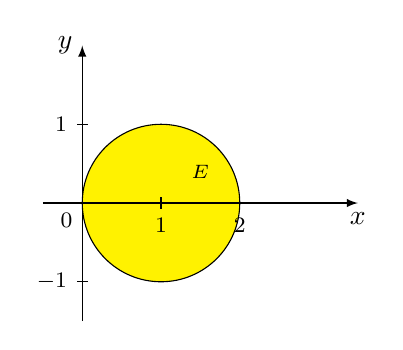
\begin{tikzpicture}[>=latex]
        \draw[fill=yellow] (1,0) circle (1);
        %x axis
        \draw[->] (-0.5,0) -- (3.5,0) node[below] {$x$};
        \foreach \x in {1,2}
        \draw[shift={(\x,0)}] (0pt,2pt) -- (0pt,-2pt) node[below] {\footnotesize $\x$};
        %y axis
        \draw[->] (0,-1.5) -- (0,2) node[left] {$y$};
        \foreach \y in {-1,1}
        \draw[shift={(0,\y)}] (2pt,0pt) -- (-2pt,0pt) node[left] {\footnotesize $\y$};
        \node[below left] at (0,0) {\footnotesize $0$};
    
        \node[font=\scriptsize] at (1.5,0.4) {$E$};
    \end{tikzpicture}
\end{multicols}

\subsection{Stokesova věta}
Užitím Stokesovy věty spočítejte 
$\iint\limits_{(M)} \text{rot} \vec{F} \dif \vec{S}$, kde $\vec{F} (x, y, z) = (xy^2, -x^2 y, xyz)$ a $M$ je část plochy
$z(x,y) = 1- x^2 - y^2$ nad rovinou $xy$ orientovaná nahoru.